\cleardoublepage
\chapter{Results}
%\label{ch:chapter1}
\label{makereference}
\section{Reconfigurable platform}
The architecture described in the previous section has been implemented using the VHDL language. To test its correct operation, the Vivado environment and the Virtex 690T FPGA \ref{basic} have been used. Although it is not a radiation-protected FPGA, the architecture of this algorithm is scalable so that its adaptation to other sensor sizes or FPGAs should not be a problem.
\begin{table}
\begin{center}
 \begin{tabular}{|c|c|c|c|c|c|} 
 \hline
 Part number & Slices & Logic cells & Flip-Flops & BRAM & DSP Slices \\
 \hline
 XCE7VX690T & 108,300 & 693,120 & 866,400 & 1,470Kb & 3,600\\
 \hline
\end{tabular}
\end{center}
\caption{Basic specifications of the Virtex 690T FPGA}
\label{basic}
\end{table}
\section{Hyperpectral image datasets}
Two hyperspectral images have been used for the work, one taken by the HYDICE sensor and the other by the AVIRIS sensor. Both images are commonly used as reference in hyperspectral applications. 
\\
\\
In the field of the scene captured by HYDICE, 15 panels of different sizes were placed on a field in a 3 x 5 meter configuration. The following images show a false color image with the bands $50$, $37$, and $17$ as red, green and blue respectively \cite{feng_hyperspectral_2020} and the location of the panels as detected by software.
\begin{figure}[!ht]
\begin{minipage}[t]{2.4in}
\begin{tabular}[b]{c|c}\hline
      Horizontal res & 64 \\ \hline
      Vertical res & 64 \\ \hline
      Bands & 210 (169*)\\ \hline
      Spectral res & 400 - 2500nm \\ \hline
      Spatial res & 1,56meter/pixel \\ \hline
      Size & 1,6 MB\\ \hline
    \end{tabular}
\end{minipage}
\begin{minipage}[t]{0.28\linewidth}
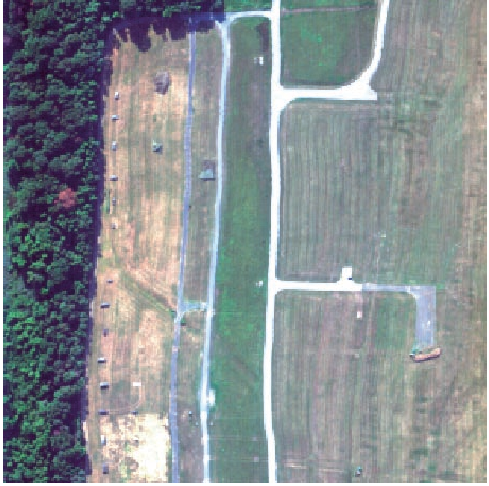
\includegraphics[width=\linewidth]{figures/hydice_bad.png}
\end{minipage}
\begin{minipage}[t]{0.28\linewidth}
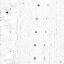
\includegraphics[width=\linewidth, frame]{figures/hydice_rx.png}
\end{minipage}
    \caption[HYDICE sensor information and used dataset]{HYDICE sensor information \cite{hydice_sensor}, image in false color and anomaly map. *In this work, images and results are reported for 169 bands}
  \end{figure}
  %https://www.indexdatabase.de/db/s-single.php?id=84
\\
\\
The image taken by the AVIRIS sensor was taken on September 16, 2001, five days after the terrorist attacks that brought down the WTC towers and its surrounding buildings. The spatial resolution of this image is very high because a very low altitude flight was performed. Along with the false color image, an image with the anomalies detected by software is provided. To ease the recognition of these anomalies, a circle has been painted around each group of anomalues for the first 30.
\begin{figure}[!ht]
\begin{minipage}[t]{2.4in}
	\begin{tabular}[b]{c|c}\hline
      Horizontal res & 614 \\ \hline
      Vertical res & 512 \\ \hline
      Bands & 224 \\ \hline
      Spectral res & 360 - 2500nm \\ \hline
      Spatial res & 1,7meter/pixel \\ \hline
      Size & 140 MB\\ \hline
    \end{tabular}
\end{minipage}
\begin{minipage}[t]{0.28\linewidth}
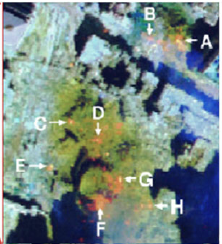
\includegraphics[width=\linewidth]{figures/wtc_bad.png}
\end{minipage}
\begin{minipage}[t]{0.28\linewidth}
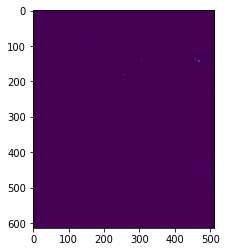
\includegraphics[width=\linewidth, frame]{figures/wtc_rx.png}
\end{minipage}
    \caption[AVIRIS sensor information and used dataset]{AVIRIS sensor information \cite{aviris_sensor}, image in false color and anomaly map}
  \end{figure}
  %https://www.indexdatabase.de/db/s-single.php?id=28
\\
\\
\section{Adequacy of approximation}
\subsection{Floating point}
The results provided by the floating point version of this system are the same as those provided by the equivalent software version, so it can be considered valid.

\subsection{Fixed point}
The fixed point version of the system is an approach to the floating point system with the intention of maintaining the highest possible accuracy with limited use of resources.
Therefore, the results are different and an assessment of their accuracy must be made. For this purpose, three metrics have been used.
\\
\\
In the first and simplest, it has been verified that the number of detected anomalies can be found in the first x positions in both results, regardless of the order.
\\
\\
Extending the previous strategy, it has been checked for the non-coinciding elements, if any neighbor has been detected in the environment. A neighbor is defined as an adjacent pixel, both in a straight line and in diagonal.
\\
\\
Finally, the first strategy has been extended again, this time it has been checked if for the non-coincidences an anomaly with a spectral similarity of less than 5 degrees has been found.
%https://www.harrisgeospatial.com/docs/SpectralAngleMapper.html
\paragraph{Spectral similarity}
The Spectral Angle Mapper (SAM) is a physics-based spectral classification that uses an n-D angle to match pixels with reference spectra. The algorithm (see \autoref{sam}) determines the spectral similarity between two spectra by calculating the angle between the spectra and treating them as vectors in a space with a dimensionality equal to the number of bands. This technique, when used in calibrated reflectance data, is relatively insensitive to the effects of illumination and albedo.
\pagebreak
\begin{figure}[h!]
\begin{minipage}[t]{0.5\linewidth}
\centering
\[\alpha = \cos^{-1}\left ( \frac{\sum\limits^{nb}_{i=1}{t_{i}r_{i}}}{\left ( \sum\limits^{nb}_{i=1}{t_{i}^2} \right )^{1/2}\left ( \sum\limits^{nb}_{i=1}{r_{i}^2} \right )^{1/2}} \right )\]
\label{sam}
\end{minipage}
\begin{minipage}[t]{0.05\linewidth}
\end{minipage}
\begin{minipage}[t]{0.45\linewidth}
\vspace{0.7cm}
$\alpha$ = spectral angle between vectors
\\
nb = number of spectral bands
\\
t = target pixel
\\
r = reference pixel
\end{minipage}
\caption{Spectral Angle Mapper algorithm}
\end{figure}
\\
\\
\subsection{Results for HYDICE}
Every pixel is found in the same order in reference and simulated calculations. Also, since those pixels are found equally, it is obvious that they are also found as neighboring pixels and are spectrally similar. Since it is an image taken to test the sensor, the targets are big and clear, and the image is quite easy to analyze.
\\
\\
\subsection{Results for AVIRIS}
The WTC image is more complex and the detection of exact pixels and neighbors quickly falls. However, the spectral signatures match for the most part, especially considering the number of real hot spots found in the image. Therefore, the results can also be taken as successful.
\pagebreak
\begin{figure}[H]
\centering
  \centering
  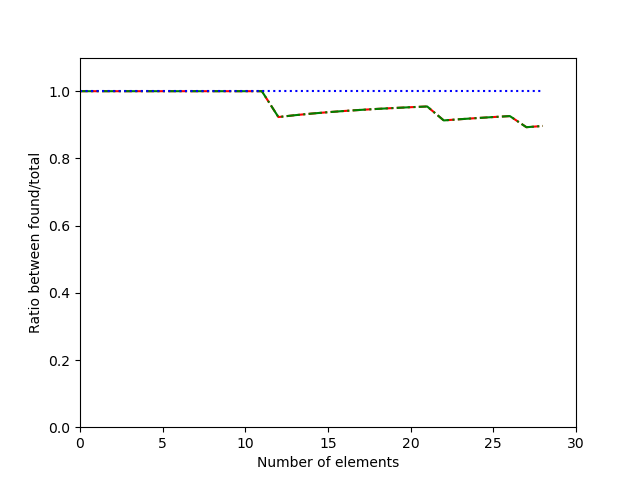
\includegraphics[width=\linewidth-1.5in]{figures/hydice.png}
  %\label{fig:sub1}
\begin{minipage}{.35\textwidth}
  \centering
  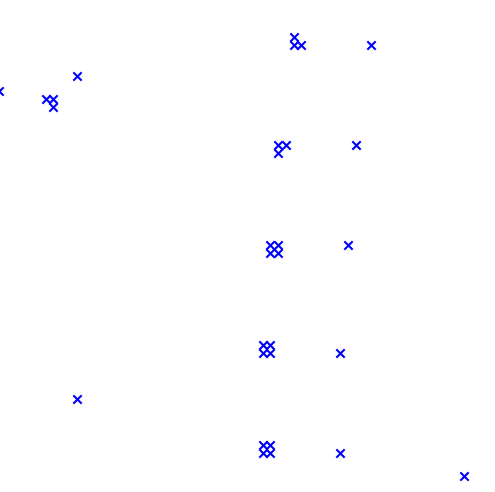
\includegraphics[width=\linewidth, frame]{figures/hydice_ref.png}
  %\caption{First 30 reference anomalies}
  %\label{fig:sub1}
\end{minipage}
\begin{minipage}{.35\textwidth}
  \centering
  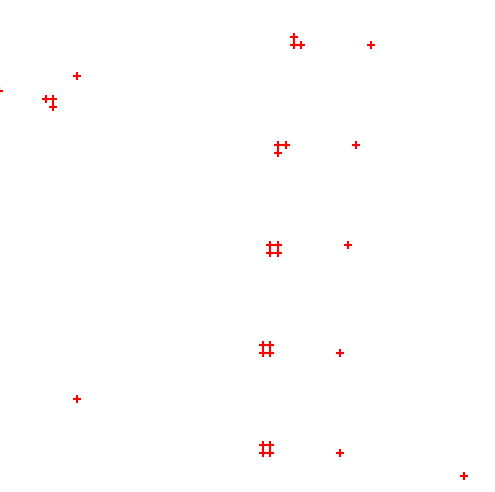
\includegraphics[width=\linewidth, frame]{figures/hydice_tar.png}
  %\caption{First 30 detected anomalies}
  %\label{fig:sub2}
\end{minipage}
\caption[Results for the HYDICE dataset]{A diagram showing similarities between referenced and achieved results and reference and achieved results mapped as in the original image for the HYDICE dataset}
\label{fig:hy_3}
\end{figure}
\newpage
\begin{figure}[H]
\centering
  \centering
  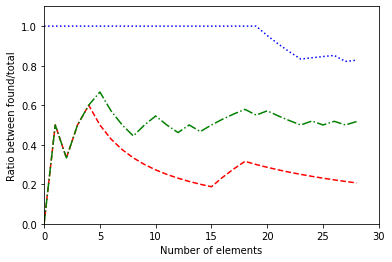
\includegraphics[width=\linewidth-1.5in]{figures/wtc.png}
  %\label{fig:sub1}
\begin{minipage}{.35\textwidth}
  \centering
  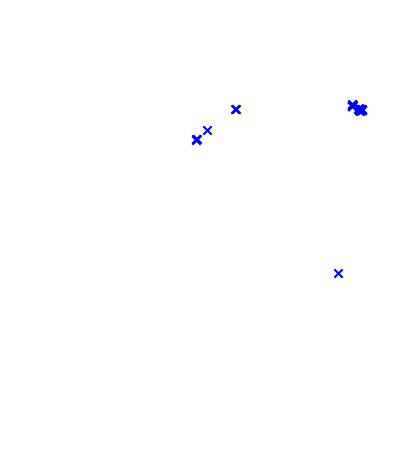
\includegraphics[width=\linewidth, frame]{figures/wtc_ref.png}
  %\caption{First 30 reference anomalies}
  %\label{fig:sub1}
\end{minipage}
\begin{minipage}{.35\textwidth}
  \centering
  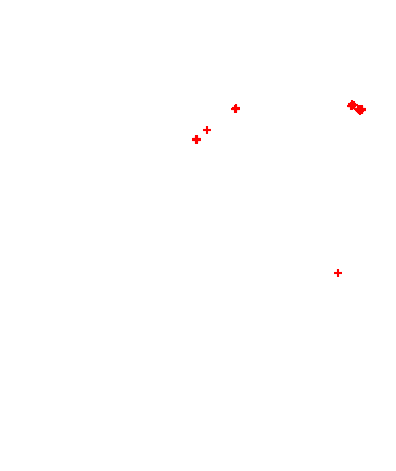
\includegraphics[width=\linewidth, frame]{figures/wtc_tar.png}
  %\caption{First 30 detected anomalies}
  %\label{fig:sub2}
\end{minipage}
\caption[Results for the AVIRIS dataset]{A diagram showing similarities between referenced and achieved results and reference and achieved results mapped as in the original image for the AVIRIS dataset}
\label{fig:av_3}
\end{figure}
\pagebreak

\noindent\begin{minipage}{\textwidth}
It should be noted that the shift values within the calculations have been adapted for each image with the intention of detecting the greatest number of anomalies possible, so that the results obtained in a real system will be slightly lower. Even so, the values between the two images are quite similar, despite the great difference between the data they represent.
\\
In addition, since it is a reconfigurable system, these values can be modified after the system is put into operation, both to accept a wider range of images, and to obtain more accurate results.
\end{minipage}

\section{Computational efficiency}
When evaluating performance, both resources used (\autoref{res_res}) and processing time (\autoref{res_lat}) must be assessed. These data are given both in those obtained for the two sensors and according to their characteristics, more specifically number of bands and pixels.
\\
It should be noted that performance data has been obtained by ignoring the input and output of data, which is often the bottleneck in this type of system.
\\

\begin{table}[h!]
\begin{center}
 \begin{tabular}{|c|c|c|c|c|} 
 \hline
 Module & LUT & Register & BRAM & DSP \\ [0.5ex] 
 \hline\hline
 Inverse & $410*bands+3484$ & $316*bands+10427$ & $<bands$ & $10*bands$\\ 
 \hline
 Mean subtraction & $bands+41$ & $136$ & $0$ & $1$\\ 
 \hline
 Matrix multiplication & $80*bands+75$ & $91*bands+223$ & $pixels/64$ & $4*bands$\\ 
 \hline
 Sort results & $186$ & $176$ & $0$ & $0$\\ 
 \hline
\end{tabular}
\end{center}
\label{res_res}
\caption[FPGA resource usage overview]{FPGA resources used in relation to number of bands and number of pixels}
\end{table}

\begin{table}[h!]
\begin{center}
 \begin{tabular}{|c|c|} 
 \hline
 Stage & Latency \\ [0.5ex] 
 \hline\hline
 Inverse & $\mathcal{O}(bands+bands^2) = \mathcal{O}(bands^2)$\\ 
 \hline
 Mean subtraction & $\mathcal{O}(1)$\\
 \hline
 Matrix multiplication & $\mathcal{O}(bands*pixels+bands)$\\
 \hline
 Sort results & $\mathcal{O}(2*bands) = \mathcal{O}(bands)$\\
 \hline
\end{tabular}
\end{center}
\label{res_lat}
\caption[Implementation latency overview]{Latency between end of previous module and end of current one}
\end{table}

Finally, the total resource utilization for both datasets and processing time is also given in \autoref{muerome}.
\begin{table}[h!]
\begin{center}
 \begin{tabular}{|c|c|c|c|c|} 
 \hline
  & Hydice & Aviris\\ [0.5ex] 
 \hline\hline
 LUT & 224.363 & 296.155\\ 
 \hline
 Register & 98.470 & 126.274\\ 
 \hline
 BRAM & 629 & 133\\ 
 \hline
 DSP & 2.371 & 3.141\\ 
 \hline
 Frecuency & 5,5 ns & 5,5 ns\\ 
 \hline
 Cycles & 1.443.418 & 140.927.349\\ 
 \hline
 Full computation & 7,938799 milliseconds & 775,10042 milliseconds\\ 
 \hline
\end{tabular}
\end{center}
\label{muerome}
\caption[Final resource and time results for the implementation]{Resource and processing time for both datasets}
\end{table}